\documentclass{article}

\input{../../../latex_preambule_style/preambule}
\input{../../../latex_preambule_style/styleCourslycee}
\input{../../../latex_preambule_style/styleExercices}
%\input{../../latex_preambule_style/styleCahier}
\input{../../../latex_preambule_style/bas_de_page_seconde}
\input{../../../latex_preambule_style/algobox}



%%%%%%%%%%%%%%%  Affichage ou impression  %%%%%%%%%%%%%%%%%%
\newcommand{\impress}[2]{
\ifthenelse{\equal{#1}{1}}  %   1 imprime / affiche  -----    0 n'affiche pas
{%condition vraie
#2
}% fin condition vraie
{%condition fausse
}% fin condition fausse
} % fin de la procédure
%%%%%%%%%%%%%%%  Affichage ou impression  %%%%%%%%%%%%%%%%%%



%%%%%%%%%%%%%%%  Indentation  %%%%%%%%%%%%%%%%%%
\parindent=0pt
%%%%%%%%%%%%%%%%%%%%%%%%%%%%%%%%%%%%%%%%%%%%%%%%



\begin{document}

\begin{tikzpicture}
\tkzTabInit[lgt=1,espcl=2]{ $x$ / 1,$f $ / 2}
{ $-5$ ,$-2$,2,5}
\tkzTabVar{+/$4$,-/$-1$,+/$3$,-/$1$ }
\end{tikzpicture}

\begin{tikzpicture}
\tkzTabInit[lgt=1,espcl=2]{ $x$ / 1,$g $ / 2}
{ $-4$ ,$-2$,3,7}
\tkzTabVar{-/$1$,+/$7$,-/$2$,+/$5$ }
\end{tikzpicture}

\begin{tikzpicture}
\tkzTabInit[lgt=1,espcl=2]{ $x$ / 1,$h $ / 2}
{ $1$ ,2,5,7}
\tkzTabVar{-/$1$,+/$7$,-/$2$,+/$5$ }
\end{tikzpicture}


\end{document}